\section{Data structures}
This section will cover the language considered followed by the selected data structures which will be used for the abstract syntax tree, which will serve as the first step of our intermediate representation. Furthermore it will cover the data structures used to store the flow graph.

\subsection{The WHILE language}
For the project the \texttt{WHILE} language will be used. It is defined below.
\\\\
a ::= n | x | A[a] | $a_1$ $op_a$ $a_2$ | -a | (a)\\
b ::= true | false | $a_1$ $op_r$ $a_2$ | $b_1$ $op_b$ $b_2$ | !b | (b)\\
S ::= x :=a; | skip; | A[$a_1$]:= $a_2$; | read x; | read A[a]; | write a; | S1 S2 | if b then S1 else S2 fi | while b do S od\\
L ::= $\epsilon$ | high | low\\
D ::= L int x; | L int A[n]; | $\epsilon$ | $D_1$ $D_2$\\
P ::= program D S end\\

\subsection{Abstract syntax tree data structure}\label{section:Abstractsyntaxtreedatastructure}
\label{sec:constructing_ast}
Before any analysis can be performed on a program written in the language in the previous section it needs to be parsed into an abstract syntax tree.\\\\
We have decided that we could use an unbalanced tree for storage of our abstract syntax tree in our target programming language. Constraining the tree construction will give us the necessary check for syntax errors.
A simple tree-traversal will give us the appropriate unique label numbers - or the ability to assign labels to statements in the right order.
\\
\\
In our implementation language the statements from the \texttt{WHILE} language will be mapped into the following  
\\\\
We will have the following structures.
\begin{itemize}
	\item \textbf{Statement} - Figure~\ref{fig:statement} shows the structures of statements.
	\item \textbf{Variable} - Figure~\ref{fig:variable} shows the structures of variables.
	\item \textbf{Condition} - Figure~\ref{fig:condition} shows the structures of conditions.
	\item \textbf{Expression} - Figure~\ref{fig:expression} shows the structures of expressions.
\end{itemize}
Declarations will be handled separately from statements, and will be held in a dedicated declarations list until needed. Only one constraint exists for declarations: Their identifiers must be unique.

\begin{figure}[h]
	\centering
	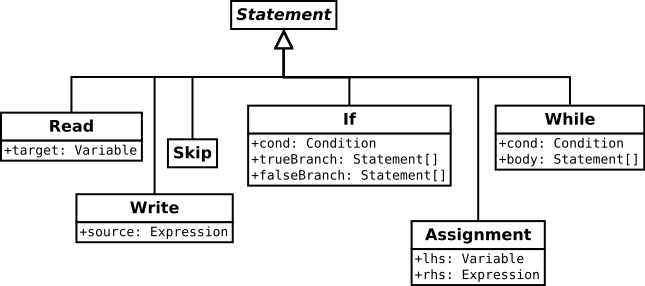
\includegraphics[scale=0.5]{../fig/Statement}
	\caption{Statement}
	\label{fig:statement}
\end{figure}

\begin{figure}[h]
	\centering
	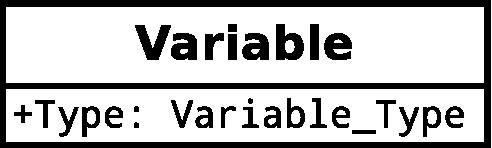
\includegraphics[scale=.3]{../fig/Variable}
	\caption{Variable}
	\label{fig:variable}
\end{figure}

\begin{figure}[h]
	\centering
	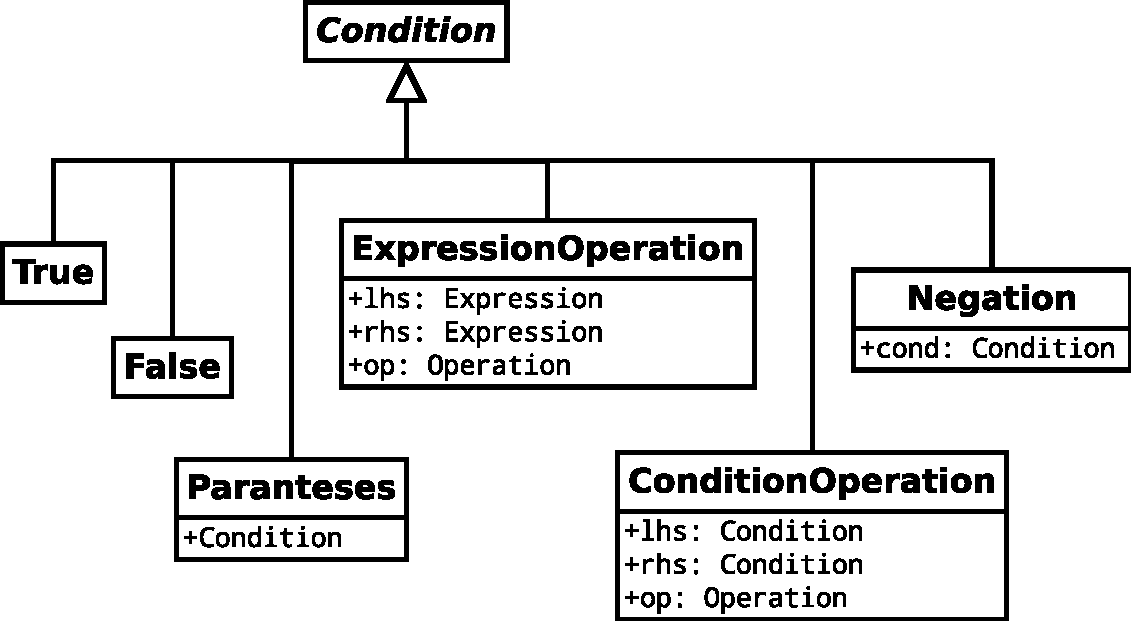
\includegraphics[scale=.3]{../fig/Condition}
	\caption{Condition}
	\label{fig:condition}
\end{figure}

\begin{figure}[h]
	\centering
	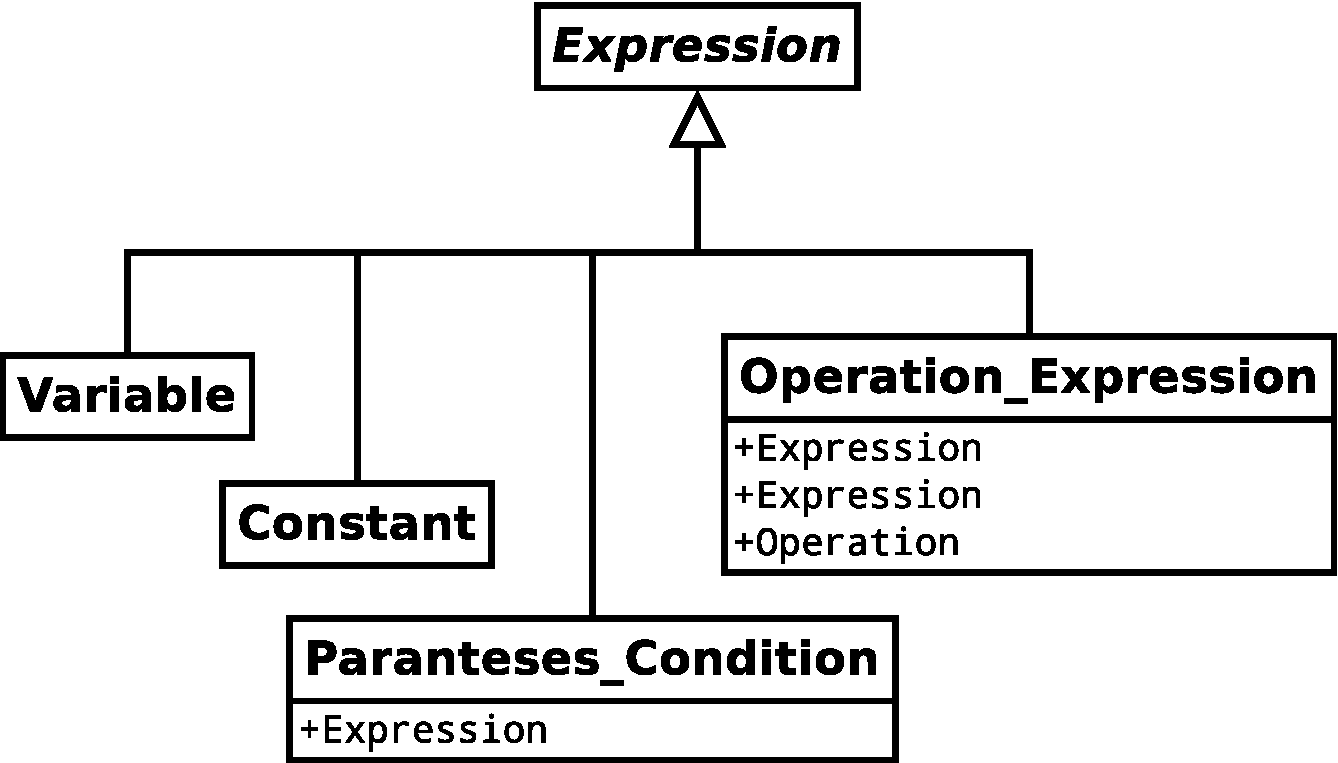
\includegraphics[scale=.3]{../fig/Expression}
	\caption{Expression}
	\label{fig:expression}
\end{figure}

\subsection{Flow graph data structure}
\label{sec:constructing_flow_graphs}
For the flow graph, we have chosen a network graph data structure. This gives an intuitive way of linking statements to potential paths.
\\
\\
It is convenient to transform the abstract syntax tree into a flow graph when performing an analysis. For that reason a data structure for the flow graph as well as mapping from a abstract syntax tree to a flow graph is needed 
\\
\\
Figure~\ref{fig:flowgraph} shows the data structure used to represent a flow graph. The idea is that a flow graph consists of a set of flow. Each flow is between two nodes. A source and a target node. A node can be a part of several flows. Each node contains a statement.	

\begin{figure}[h]
	\centering
	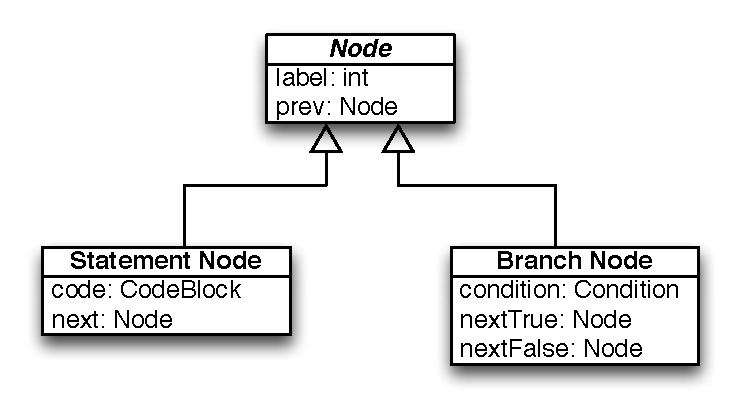
\includegraphics[scale=0.6]{../img/flow_graph}
	\caption{Data structures used to represent a flow graph}
	\label{fig:flowgraph}
\end{figure}

\subsubsection{Defining flow graphs}\label{section:CreatingFlowGraphs}
Before any analysis can take place we need to create a flow graph based on our abstract syntax tree. A flow graph should consists of the elements presented in table~\ref{table:flow_graph_definitions}.
\begin{table}
    \begin{tabular}{l | l }
    \textsl{label(S)} & The set of nodes of the flow graph $S$ \\
    \hline    
    \textsl{init(S)}  & The initial node of the flow graph $S$.\\
               & Unique node where the execution of the program starts.\\
    \hline
    \textsl{final(S)}   & The final node of the flow graph $S$.\\
                 & A set of nodes where the execution of the program may terminate.\\
    \hline
    \textsl{flow(S)} & The edges of the flow graph for $S$. A set of pairs is returned. \\
	\hline
    \textsl{block(S)}   & A set of the blocks/statements in the program under inquisition.\\
    \end{tabular}
    \centering
	\caption{Function definitions}
	\label{table:flow_graph_definitions}
\end{table}
\\\\
The objective is to establish a flow graph using the abstract syntax tree. Using the intermediate representation of the abstract syntax tree, the types of different individual statements is defined. Rather than explicitly parsing the AST to a flow graph, we instead define a function for each statement and let every statement handle it's own branch by recursion using the function defined in table~\ref{table:flow_graph_functions}.

\begin{table}
\begin{tabular}{| l | l | l | l | l | l |}
\hline	
\textsl{S}                              & \textsl{labels(S)}                                    & \textsl{init(S)}     & \textsl{final(S)}  & \textsl{flow(S)}            & \textsl{blocks(S)}  \\ 
\hline
[x := a]$^\ell$                         & $\{\ell\}$                                            &$\ell$                & $\{\ell\}$ & $\emptyset$        &\{[x := a]$^\ell$\}   \\
\hline
[A[a$_1$] := a$_2$]$^\ell$          & $\{\ell\}$                                            &$\ell$                & $\{\ell\}$ & $\emptyset$      &\{[A[a$_1$] := a$_2$]$^\ell$\}\\
\hline
[skip]$^\ell$                           & $\{\ell\}$                                            &$\ell$                & $\{\ell\}$   & $\emptyset$       &\{[skip]$^\ell$\}  \\
\hline
\textsl{S}$_1$;\textsl{S}$_2$           & \textsl{labels(S$_1$)} $\cup$ \textsl{labels(S$_2$)}  & \textsl{init(S$_1$)} & {final(S$_2$)} & \textsl{flow(S$_1$)} $\cup$ \textsl{flow(S$_2$)} & \textsl{block(S$_1$)}  \\ 
&&&&$\cup$\{($\ell$,\textsl{init(S$_2$)}) | $\ell\in$\textsl{final(S$_1$)} \}& $\cup$ \textsl{block(S$_2$)}\\
\hline
if [\textsl{b}]$^\ell$ then             & $\{\ell\}$ $\cup$  \textsl{labels(S$_1$)}             &$\ell$                & \textsl{final(S$_1$)} & \textsl{flow(S$_1$)} $\cup$ \textsl{flow(S$_2$)}  & \{[\textsl{b}]$^\ell$\} $\cup$\ \textsl{block(S$_1$)} \\
  \textsl{S}$_1$ else \textsl{S}$_2$    &  $\cup$ \textsl{labels(S$_2$)}                        &                      & $\cup$ \textsl{final(S$_2$)} & $\cup$\{($\ell$,\textsl{init(S$_1$)}),($\ell$,\textsl{init(S$_2$)} \}&  $\cup$ \textsl{block(S$_2$)}\\
\hline
while [\textsl{b}]$^\ell$ do \textsl{S} & $\{\ell\}$ $\cup$  \textsl{labels(S)}                 &$\ell$                & $\{\ell\}$ & \{($\ell$,\textsl{init(S)})\} $\cup$\textsl{flow(S)}                 & \{[\textsl{b}]$^\ell$\} $\cup$\ \textsl{block(S)} \\
&&&&$\cup$ \{($\ell^{'}$,$\ell$) |  $\ell^{'}\in$ \textsl{final(S)} \}&\\
\hline
[read \textsl{x}]$^\ell$                & $\{\ell\}$                                            &$\ell$                & $\{\ell\}$ & $\emptyset$                                            &\{[read \textsl{x}]$^\ell$ \}  \\
\hline
[read A[a$_1$]]$^\ell$                & $\{\ell\}$                                            &$\ell$                & $\{\ell\}$  & $\emptyset$                                            &\{[read A[a$_1$]]$^\ell$ \}   \\
\hline
[write \textsl{x}]$^\ell$               & $\{\ell\}$                                            &$\ell$                & $\{\ell\}$  & $\emptyset$                                          &\{[write \textsl{x}]$^\ell$ \} \\
\hline
[write A[a$_1$]]$^\ell$               & $\{\ell\}$                                            &$\ell$                & $\{\ell\}$  & $\emptyset$                                          &\{[write A[a$_1$]]$^\ell$\} \\
\hline
\end{tabular}
\centering
\caption{Flow graph function definitions}
\label{table:flow_graph_functions}
\end{table}

\subsection{Program graph data structure}
Another approach for structuring a program is to use a program graph which is similar to flow graphs but instead of storing the statements in the nodes they are stored in the edges. This has some advantages in certain analysis but in general both flow graph and programs graph can be used since it is possible to convert between the two.
\\\\
In the rest of the report the focus will be on flow graphs.